% !TeX root = proposal.tex

\iffalse
Your objectives are the most important part of the proposal. 

Tell the reader what you intend to accomplish; 
	see if you can state the expected outcomes in a clear fashion so that you know, 
	and the reader knows, what you are going to have when finished.
	
What theory will you work out? 
Or what measurements will you make? 
Or what circuit will you build? 
The clearer you are with this, the higher the chances will be for knowing how to get there.
Break the Objectives down into pieces on which each of your teammates will focus. 
Show how the individual objectives create the project’s overall end objective.

Once you know what you will be doing, put the steps into a Gantt Chart.Look online for a Gantt Chart description if you need to.


\fi

\begin{figure}[H]
	\centering
	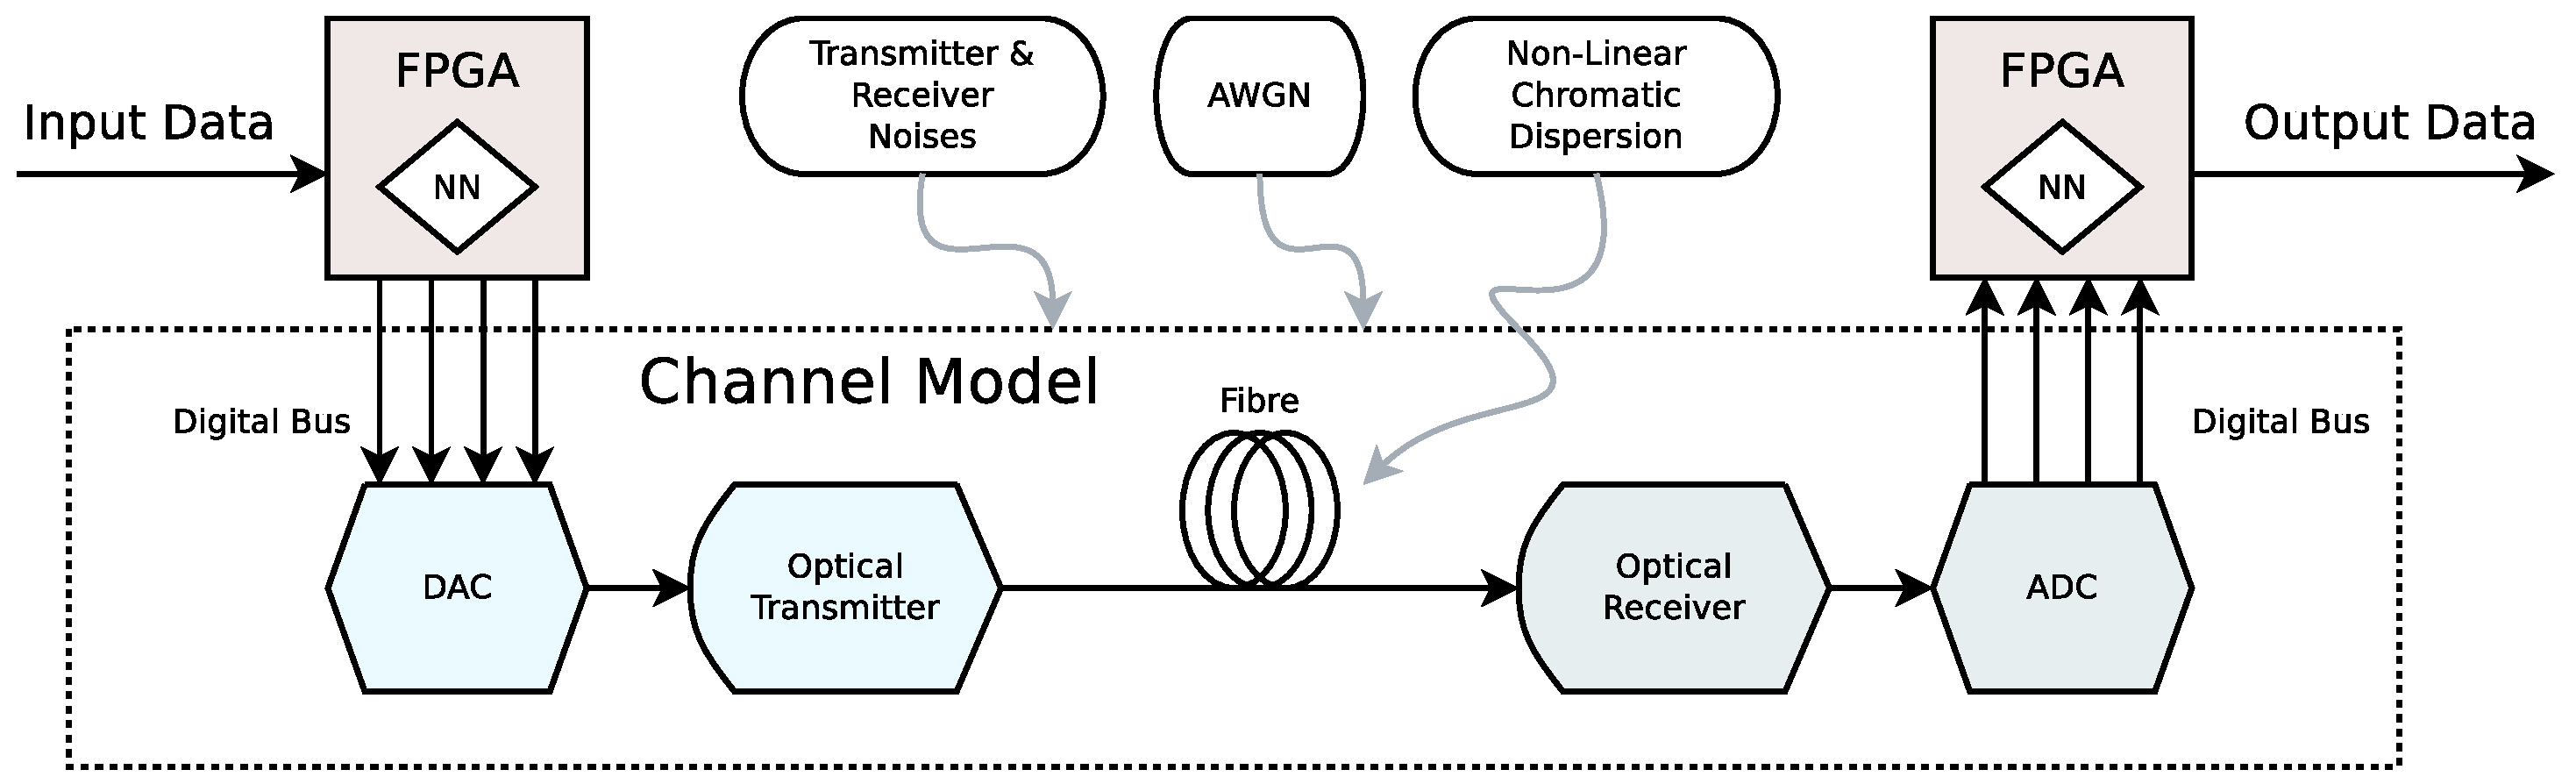
\includegraphics[width=\linewidth]{graphics/overall_diagram2.eps}
	\caption{Simplified overall system diagram with the modulator and demodulator shown as black box NN implmeneted on FPGAs}
	\label{fig:overall}	
\end{figure}

The main objective of this project is to design a suitable NN to optimize the transmission of data via a communication channel and implement it on a FPGA hardware. The channel that will be of primary focus is the optical fibre communication channel where non-linearities introduced by chromatic dispersion and photodiode detection is a major problem that needs to be overcome. The project can be broken down into individual objectives that will need to be achieved:

\begin{itemize}
    \item Choosing an Appropriate NN Architecture
    \item Simulating the Communication Channel and Proposed Transmitter/Receiver
    \item Implementing the NN on a FPGA
    \item Training and Testing the System using an Optical Fibre Communication System
\end{itemize}

\subsection{Choosing an Appropriate Neural Network Architecture}

The modulation scheme as well as the encoding of the bits will be learned for the specific communication channel by a NN at the transmitter. Likewise, at the receiving end of the communication system, a separate NN will decode the received signal into a stream of bits. A simple NN sometimes referred to a Multi-Layer Perceptron (MLP) is shown in Fig X.X. This example shows a very simple MLP with an input layer followed by 3 layers. The last layer is known as the output layer as it produces the output. The 2 layers in-between the input and output layers are referred to as hidden layers. This particular MLP takes a 3 valued vector $\boldsymbol{x}$ and produces a single real valued output $\hat{y}$. In addition to this it is fully connected meaning that each node (represented by a circle in the figure) receives input from each of the nodes in the previous layer. Each layer is characterized by it's weight matrix $\boldsymbol{W}$ as well as it's activation function. During training it is $\boldsymbol{W}$ that is learnt to obtain the relationship between input and output.
\\
\\
The study carried out in \autocite{8664650} features a Convolutional Neural Network (CNN) at the transmitting and receiving end of the communication system. Similar to our own project, the paper describes an end to end neural network implementation for the communication system. The channel used in the simulations is an Additive White Gaussian Noise (AWGN) model and does not consider potential non-linearities introduced in the channel. On the contrary, \autocite{6975096} describes a Multi-Layer Perceptron (MLP) based Non-Linear Equalizer(NLE) at the receiver for an optical communication system. As this paper, clearly discusses the optical communication channel, it may be useful in deciding on a suitable neural network at the transmitter. It should be noted that the paper describes an equalizer and not a demodulator/decoder. 
\\
\\
When deciding on a NN we must not only choose an approapriate architecture but also choose the most optimal activation function. The activation function is key as it is this that introduces non-linearity into the learnt model. Some of the most commonly used activation fucntions are the Rectified Linear Unit (ReLu), hyperbolid tangent (tanh), sigmoid and the leaky ReLu. These are illustrated in Fig. X.X.
\\
\\
Further research and literature review needs to be done into different architectures that are available and the requirements that need to be met by the transmitter and receiver of the communication channel. Depending on the chosen neural network architecture, a suitable FPGA will need to be decided on as well. Different architectures may demand different levels of hardware resources.

\subsection{Simulating the Communication Channel and Proposed Transmitter/Receiver}

An optical communication channel is comprised of a transmitter, receiver and the optical fibre connecting the two together. In order to simulate this communication channel, the mathematical representation of the signal at each stage of the channel needs to be established. The signal that enters the optical fibre is described by its electrical field of the EM field, known as its optical field and is expressed mathematically in the time domain as: 

\begin{equation}
    A(t, z) = |A(t,z)|e^{j\phi(t,z)}
\end{equation}
\\
\\
where z is the distance along the fibre and t is the time. A(t,z) is a phasor incorporating the optical amplitude $|A(t,z)|$ and optical phase $\phi(t,z)$. 
\\
\\
The signal suffers from chromatic dispersion as it traverses through the optical fibre, resulting in different frequency components of the signal being delayed by different amounts. For simulation simplicity, this effect will be simulated in the frequency domain due to a linear time delay vs frequency and can be expressed by the following mathematical expression:
\begin{equation}\label{opticalField}
    A(\omega,L) = A(\omega,0)e^{j\frac{1}{2}\beta_z\omega^2L}
\end{equation}
where $\omega$ is angular frequency, $\beta_z$ is the group velocity dispersion and L is the fibre length.
\\
\\
At the receiver, photodetection is carried out by using the proportional relationship between the output voltage and power of the signal which in turn is proportional to the square of the magnitude of the optical field, resulting in the following mathematical expression.

\begin{equation}
    V_{out}(t) = |A(t,L)|^2
\end{equation}
    where A(t,L) is the inverse Fourier transform of eqn.\ref{opticalField}.
\\
\\
To complete the mathematical representation of the signal through an optical channel, the receiver noise is applied to the photodetected signal. This is in the form of white Gaussian noise (randomly generated volatages $\DeltaV(t)$, which are generated with a normal distribution) which is added to both the model shot noise and the thermal noise. This voltage waveform is then the representation of the signal after it leaves the receiver.
\\
\\
The transmitting and receiving end as well as the channel itself need to be simulated as a channel model. The neural networks will most likely be implemented using the TensorFlow package with python. The different characteristics of the channel need to be included in the model to ensure that it sufficiently represents how a transmitted signal would be altered by a real optical fibre communication channel. \autocite{8433895} describes a potential model for the optical communication system. This model includes a low-pass filter (LPF) to account for the finite bandwidth of read hardware, a digital to analogue converter (DAC), an analogue to digital converter (ADC), a Mark-Zehnder modulator (MZM), photo-conversion by a photodiode, Gaussian noise as well as the optical fibre transmission itself. We will need to decide on the communication channel configuration that we wish to simulate as well as the data-rate of the communication system. 

This simulation could replace channel model which would look as a back box while training Neural Networks.

\subsection{Implementing the Neural Networks on a FPGA}

Implementing Neural Network on FPGA raises a number problems that need to be considered.
 
\subsubsection{Data structures}
FPGA internal data structure has a tradeoff between performance and accuracy, as some of neural network can operate on smaller numbers without losing much accuracy \autocite{8330546}, with huge improvements in speed and need of FPGA resources \autocite{omondi_rajapakse_2006}. 

Thoughtout different research papers, a number of data structures are proposed, some use a mix for different layers:
\begin{itemize}
	\item Full-Precision Floating-point (32bit)
	\item Half-Precision Floating-point (16bit) \autocite{6927383,8108073}
	\item Mini-Precision Floating-point (8bit) \autocite{6927383}
	\item Nibble-Precision Floating-point (4bit) \autocite{6927383}
	\item Quantized Number (up to 8bit) \autocite{8702332,8280163,8330546}
	\item Binary Matrix or Vector \autocite{9039366,8280163,7929192}
\end{itemize}

\subsubsection{Required FPGA resources}
 Depending on implemented Neural Network, its size, used data structure, a suitable FPGA board needs to selected. 
 
 Option to use multiple FPGA boards that would be linked with fast communication protocols will be also considered, including overall board architecture.

\subsubsection{FPGA Memory}
Depending on Neural Network size and required bandwidth, internal or external memory might be used. Internal memory is limited in size, and might cause issues with maximum internal FPGA connections \autocite{7929192}.
External memory increases complexity and requires high bandwidth bus. There are a number of improvements that can be used for NN architecture such a memory data compression to allow avoid bandwitdth issues \autocite{9012821}.

\subsubsection{Sigmoid optimisations}
Sigmoid function is used in Neural Networks (such as ANN) as the activation function, and is one of main nerual network blocks. It uses Sigmoid function \autoref{sigmoid} which uses complex mathematical expression.
\begin{equation}\label{sigmoid}
    f(x) = \frac{1}{1+e^{-x}}
\end{equation}

A novel approximation is available which uses about a third of FPGA resources \autocite{9027479}.

\subsubsection{Neural Network optimisations in FPGA} 
There are a number of research papers that include some optimisations to implement Neural Networks on FPGA: 
\begin{itemize}
	\item Feed forward ANN on FPGA \autocite{7011454}
	\item ANN based PID controller on FPGA \autocite{5328349}
\end{itemize}
Further research will be done to find optimal implementation of Neural Network in HDL.

\subsection{Training and Testing the System using an Optical Fibre Communication System}

If time and circumstance permits the project could conclude by testing the designed system using an experimental setup to simulate the communication channel as opposed to a computer model. This would bring light to discrepancies between the real-life setup and the simulated model. As well as that, it would validate that the design works as well in an experimental setup as it does in simulation. The neural network could be trained at different lengths of fibre and observed to see how the learned parameters as well as the bit error rate differ to traditional methods of encoding/decoding. 
